\section{Regression}
\renewcommand{\loadeq}[1]{\ExecuteMetaData[../equations/regression.tex]{eq#1}}

\begin{frame}
\begin{figure}[ht!]
\ifisPPT
\noindent\makebox[\textwidth]{\includegraphics[keepaspectratio=true,width=\paperwidth]{../figures/regression/basicLSE.jpg}}
\else
\includegraphics[keepaspectratio=true,width=6in]{./figures/regression/basicLSE.jpg}
\fi
\centering
\caption{Basic LSE}
\label{fig:basicLSE}
\end{figure}


\end{frame}

\begin{frame}
\frametitle{Basic Regression}
\loadeq{ExLinEqu}
\loadeq{LSEE2}
\loadeq{LSEE2b}
\loadeq{LSEPD}
\end{frame}

\begin{frame}
% This figure was generated by ./scripts/modeling/plot_ExCapData.m
\begin{figure}[ht!]
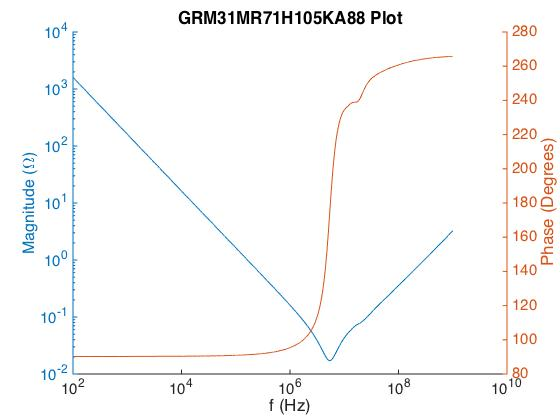
\includegraphics[keepaspectratio=true,width=6in]{./figures/modeling/exCapData.jpg}
\centering
\caption{GRM31MR71H105KA88 Capacitor Data}
\label{fig:exCapData}
\end{figure}

\end{frame}

\begin{frame}
\loadeq{levyGs}
\loadeq{LevyL}
\loadeq{LevyS}
\loadeq{LevyT}
\loadeq{LevyU}
\end{frame}

\begin{frame}
\loadeq{fullModelM}
\end{frame}

\begin{frame}
\loadeq{LevyNC}
\loadeq{LevyAns}
\end{frame}

\begin{frame}
% Run /scripts/regression/run_levy_iter.m with NumDeg = 3, DenDeg = 3, and iterations = 1.
\begin{figure}[ht!]
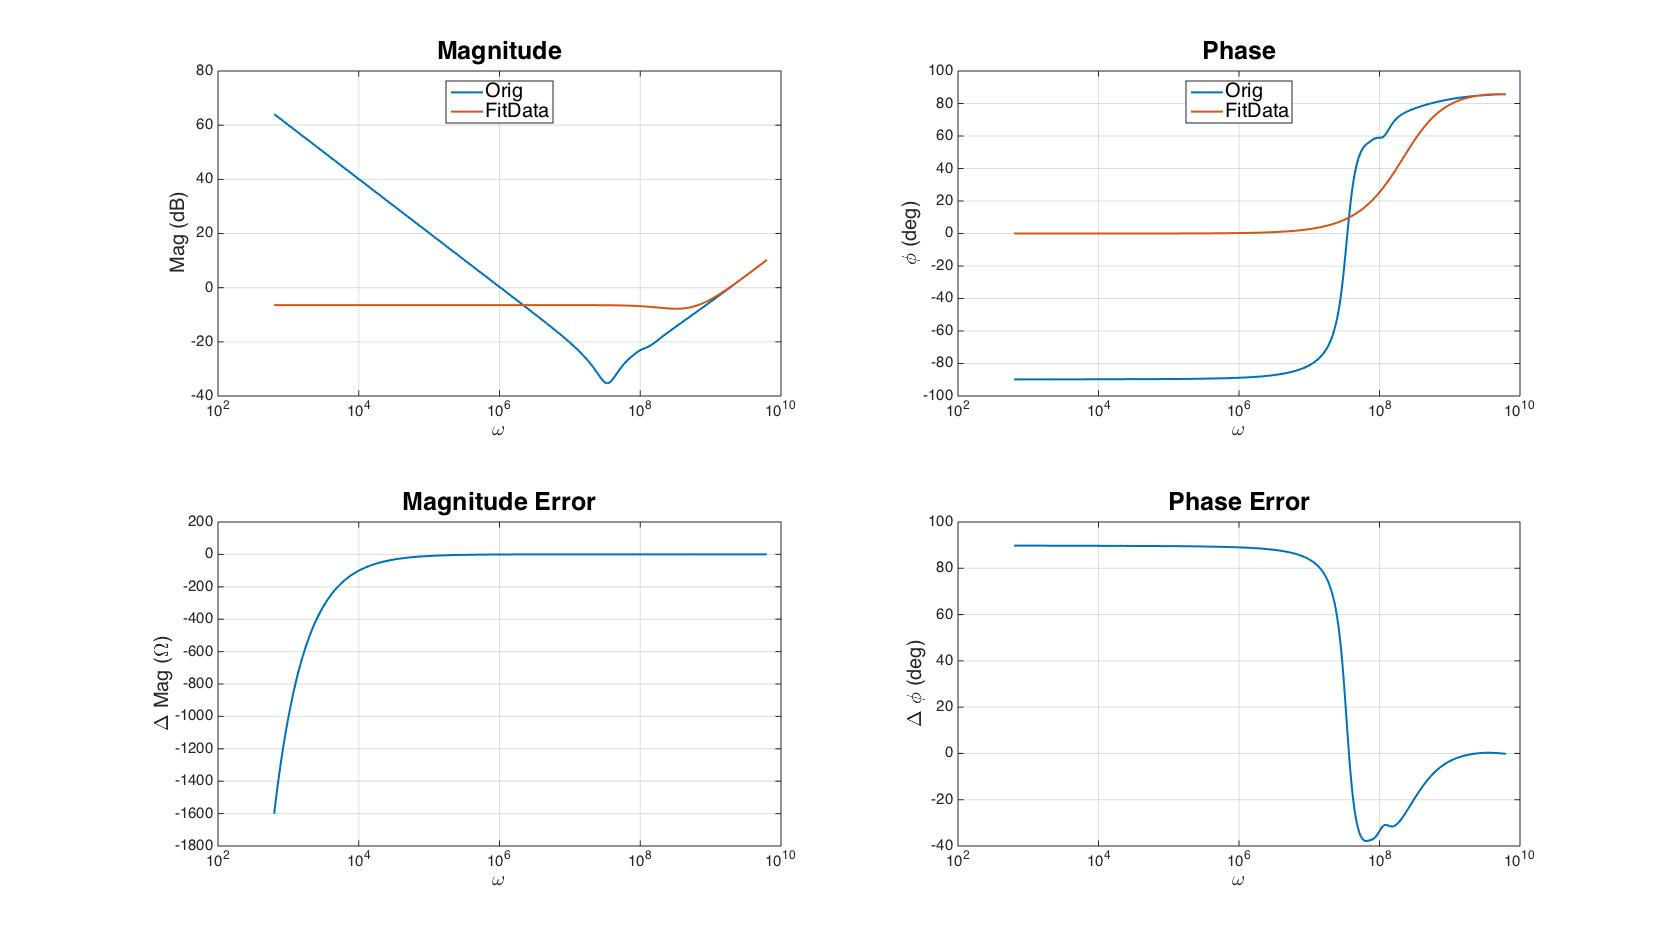
\includegraphics[keepaspectratio=true,width=6in]{./figures/regression/levy.jpg}
\centering
\caption{Levy's Technique}
\label{fig:levy}
\end{figure}


\end{frame}

\begin{frame}
\loadeq{iterWeight}
\loadeq{iterErr}
\end{frame}

\begin{frame}
\begin{figure}
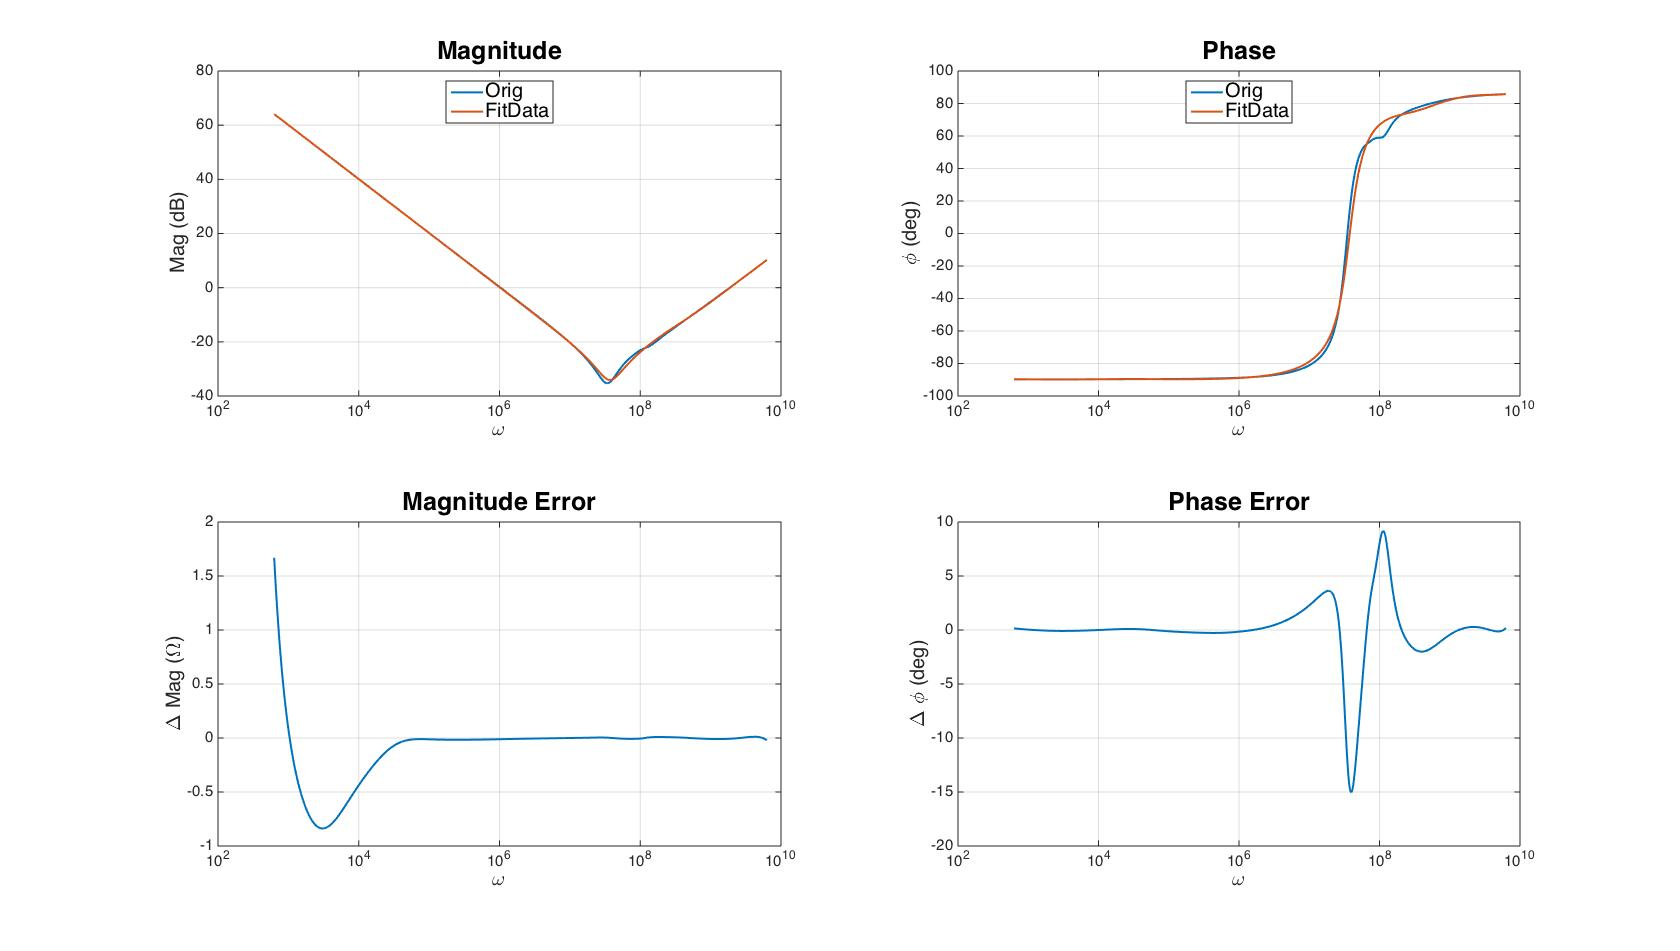
\includegraphics[keepaspectratio=true,width=6in]{./figures/modeling/levyIter.jpg}
\centering
\caption{LSE + Iteration}
\label{fig:levyIter}
\end{figure}

\end{frame}

\begin{frame}
\begin{figure}[ht!]
\ifisPPT
\noindent\makebox[\textwidth]{\includegraphics[keepaspectratio=true,width=\paperwidth]{../figures/regression/fullModel.jpg}}
\else
\includegraphics[keepaspectratio=true,width=2in]{./figures/regression/fullModel.jpg}
\fi
\centering
\caption{6 Term Model}
\label{fig:fullModel}
\end{figure}

\end{frame}

\begin{frame}
\loadeq{fullModelImpedance}
\loadeq{fullModelPoly}
\end{frame}

\begin{frame}
\begin{figure}[ht!]
\ifisPPT
\noindent\makebox[\textwidth]{\includegraphics[keepaspectratio=true,width=\paperwidth]{../figures/regression/fullModel_BadOutput.jpg}}
\else
\includegraphics[keepaspectratio=true,width=6in]{./figures/regression/fullModel_BadOutput.jpg}
\fi
\centering
\caption{6 Term Model: Bad Initilization}
\label{fig:fullModel_BadOutput}
\end{figure}

\end{frame}

\begin{frame}
\loadeq{FullModelBadOut}
\end{frame}

\begin{frame}
\loadeq{FullModelBadIn}
\end{frame}

\begin{frame}
\loadeq{FullModelGoodIn}
\end{frame}

\begin{frame}
\begin{figure}[ht!]
\ifisPPT
\noindent\makebox[\textwidth]{\includegraphics[keepaspectratio=true,width=\paperwidth]{../figures/regression/fullModel_GoodOutput.jpg}}
\else
\includegraphics[keepaspectratio=true,width=6in]{./figures/regression/fullModel_GoodOutput.jpg}
\fi
\centering
\caption{6 Term Model: Good Initilization}
\label{fig:fullModel_GoodOutput}
\end{figure}

\end{frame}

\begin{frame}
\begin{figure}[ht!]
\ifisPPT
\noindent\makebox[\textwidth]{\includegraphics[keepaspectratio=true,width=\paperwidth]{../figures/regression/fullModel_Rel.jpg}}
\else
\includegraphics[keepaspectratio=true,width=6in]{./figures/regression/fullModel_Rel.jpg}
\fi
\centering
\caption{6 Term Model: Relative Error}
\label{fig:fullModel_Rel}
\end{figure}

\end{frame}

